\documentclass[a4paper,11pt]{scrreprt}                       % default is A4 paper style and 11pt font size


%%%%%%%%%%%% version history %%%%%%%%%%%%%%%%%%%%%%%%%%%%%%%%%%%

%26.03.2017:    corrections for the latex source-code: diacritics issues; corrected the glossaries and added listings packages; added fontspec (only works with xelatex/lualatex !!!)
%2014:          put in latex version + some small additions - Florin Stoican
%2013:          content from Dan Stefanoiu
%%%%%%%%%%%%%%%%%%%%%%%%%%%%%%%%%%%%%%%%%%%%%%%%%%%%%%%%%%%%%%%%%%%%%%%%%


%%%%%%%%%%%% macros for various paths %%%%%%%%%%%%%%%%%%%%%%%%%%%%%%%%%%%
\def \cls {./cls} 																					 % path to common latex files (change for your own relative/absolute path)
\def \pics {./pics}      																		 % path to pics files (change for your own relative/absolute path)
\def \chapters {./chapters}      														 % path to chapter files (change for your own relative/absolute path)
\def \code {./code}      													        	 % path to source code files (change for your own relative/absolute path)

% you don't have to use them but it's nicer this way
%%%%%%%%%%%%%%%%%%%%%%%%%%%%%%%%%%%%%%%%%%%%%%%%%%%%%%%%%%%%%%%%%%%%%%%%%
\usepackage{tikz}
\usepackage{pgfplots}
\usepackage{float}
\usepackage{svg}
\newcommand{\norm}[1]{\left\lVert#1\right\rVert}
%\usepackage{subfig}
% language={english/romanian} selects between the languages used in the manusript (changes, e.g., the name of the chapter)
% type={bachelor/master/phd} selects between the type of manusript (changes, e.g., the titlepage make-up)
\usepackage[language=romanian,type=bachelor]{\cls/standard} % introduces useful packages and commands(CHANGE ONLY IF YOU KNOW WHAT YOU'RE DOING)
\addbibresource{\cls/bib.bib}																% bib resource (using biblatex package, for complex stuff use the biber backend instead of bibtex
\newglossaryentry{computer}
{
  name=computer,
  description={is a programmable machine that receives input,
               stores and manipulates data, and provides
               output in a useful format}
}

\newacronym[longplural={Frames per Second}]{fpsLabel}{FPS}{Frame per Second}
\newacronym{lvm}{LVM}{Logical Volume Manager}        																	% put here all your glossary terms; only the ones actually used will appear in the glossary list of the manuscript

\begin{document}

%%%%%%%%%%%%%%%%%%%%%%% frontmatter %%%%%%%%%%%%%%%%%%%%%%%%%%%%%%%%%%%%%
\pagenumbering{roman}																				% default numbering for the frontmatter is roman

\title{Clasificare defecte într-o rețea de apă de mari dimensiuni}														% title of your manuscript
\author{Cazan Cristian-Claudiu}																				% author name
\advisor{Florin Stoican}																			% advisor name

\maketitle

% show table of contents, figures, tables and algorithms

\tableofcontents 
\printnoidxglossaries																				% \printglossaries works only if the makeindex has the correct arguments
\addcontentsline{toc}{chapter}{\listfigurename}
\listoffigures 
\addcontentsline{toc}{chapter}{\listtablename}
\listoftables
\addcontentsline{toc}{chapter}{\listalgorithmcfname}
\listofalgorithmes

\clearpage

%%%%%%%%%%%%%%%%%%%%%%% mainmatter %%%%%%%%%%%%%%%%%%%%%%%%%%%%%%%%%%%%%%
\pagenumbering{arabic}																			% default numbering for the mainmatter is arabic

% here is the text of you manuscript; you can put it directly here but it is better to include files (the main file will be more compact)
\chapter{Introducere}
\label{chap:intro}

\section{Motivația alegerii temei}
Transportul și distribuția apei reprezintă una dintre cele mai vechi preocupări inginerești de proporții, existând de mai mult de 4000 de ani. Civilizația minoică, localizată în insula Creta, este considerată a fi prima care a construit apeducte - structuri pentru transportul apei de la sursă către orașe - în 2500 î.Hr. 

Deși majoritatea popoarelor din antichitate care s-au ocupat cu construcția apeductelor întrebuințau aceste sisteme pentru irigația pământului - ocupațiile de bază de atunci fiind în strânsă legătură cu agricultura - romanii au văzut în sistemele de provizionare a apei și un potențial imens în dezvoltarea civilizației, astfel ei sunt ei care aduc cele mai mari contribuții inginerești, apeductele construite de aceștia impresionând și astăzi prin grandoarea și iscusunța cu care au fost construite.

Inovațiile în acest domeniu au suferit salturi bruște și puternice în momentul descoperirii unei noi relații matematice care transformă un parametru despre care se puteau face doar niște estimări grosiere într-o mărime bine definită și bine controlată. Istoric vorbind începutul dezvoltării științei hidraulice s-a bazat pe relația descoperită de Arhimede din Siracuza în sec III î.Hr, $F = V_{obiect} \cdot \rho_{lichid}*g$. O altă contribuție care are o deosebită importanță în domeniul tehnologiei de distribuiție a apei și nu numai o reprezintă tubul lui Pitot folosit la măsurarea vitezei fluidului, inventat de Henri Pitot în sec XVII. Din punct de vedere constructiv tubul are o formă de \textbf{L}, scufundarea acestuia într-un fluid (apă sau gaz) va determina creșterea nivelului și a presiunii până la o anumită limită \cite{klopfenstein1998air}, ecuația care guvernează depedența nivel - viteză este:
\begin{equation}
u = \sqrt{\frac{2(p_t-p_s)}{\rho}} 
\end{equation}

unde:

\begin{description}
\item u reprezintă viteza fluidului;
\item $p_t$ reprezintă presiunea de stagnare;
\item $p_s$ reprezintă presiunea statică;
\item $\rho$ reprezintă densitatea fluidului.
\end{description}

Mergând mai departe, alte contribuții importante apar din partea marilor matematicieni precum Daniel Bernoulli și Leonhard Euler, care au mărit spectrul mecanicii lui Newton și Leibniz spre aria hidraulicii și a termodinamicii. Fluidele considerate sunt incompresibile și au densitatea constantă în timp și uniform distribuită în spațiu. Bernoulli afirmă despre lichidele incompresibile că o creștere în viteză a lichidului este însoțită de o scădere a energiei potențiale a lichidului (i.e. a presiunii):
\begin{equation}
\frac{u^2}{2} + gz + \frac{p}{\rho} = c
\end{equation}

unde:
\begin{description}
\item v reprezintă viteza fluidului;
\item g reprezintă accelerația la care e supus fluidul;
\item z reprezintă elevația ștrangulației conductei;
\item p reprezintă presiunea într-un anumit punct;
\item $\rho$ reprezintă densitatea fluidului.
\end{description}

În contextul în care se dorește analiza unui caz real este important ca toate diferențele între cazurile ideale și cazurile reale să fie puse în evidență în mod matematic, astfel se particularizează ecuația generală Navier-Stokes pentru cazuri în care se cunosc anumiți parametrii ai sistemului de analizat. Spre exemplu ecuația Poisuille care modelează începutul fluxului de apă într-o conductă este \cite{elger2016engineering}:
\begin{equation}
\frac{\partial u}{\partial t} = \frac{G}{\rho} + \nu \left( \frac{\partial^2 u}{\partial t^2} + \frac{1}{r}\frac{\partial u}{\partial{r}}\right)
\end{equation}

unde:
\begin{description}
\item $u$ reprezintă viteza lichidului prin conductă
\item $t$ reprezintă timpul
\item $G$ reprezintă diferența de presiune
\item $\rho$ reprezintă densitatea lichidului
\item $\nu$ reprezintă vâscozitatea cinematică
\item $r$ reprezintă poziția
\end{description}

Se poate observa că pe măsură ce modelul matematic se apropie de realitate, complexitatea acestuia crește și pentru fiecare situație specială - spre exemplu analiza presiunii la  introducerea apei într-o conductă vs. analiza presiunii când conducta este încărcată cu apă - are nevoie de o ecuație specială sau de o particularizare a ecuației Navier-Stokes, pentru care încă nu se cunoaște dacă există soluții pentru cazul cu 3 dimensiuni și dacă soluțiile acestea sunt netede. 

Ținând cont de importanța apei în desfășurarea activităților cotidiene atât pentru oameni cât și pentru actorii importanți ai industriei, este o condiție absolut necesară ca un oraș să aibă un sistem performant de distribuție a apei. În contextul actual al dezvoltării tehnologiei este natural să folosim tehnici moderne de monitorizare a diferiților parametrii din cadrul unei rețele pentru a putea face o analiză riguroasă și eficientă cu referire nu numai la mentenanță ci și la consumul global și local în ideea îmbunătățirii și reducerii pierderilor.


\section{Expunerea problemei}

În această lucrare se va aborda problematica identificării prezenței unui defect - \textit{Fault detection} și izolarea defectului \textit{Fault isolation} apărut într-un nod al rețelei - aceasta reprezentând o simplificare deoarece un defect apare de obicei într-una din conductele rețelei legate de acel nod. Combinănd cei doi termeni obținem \textit{Fauld detection and Isolation} (FDI).

O rețea de apă poate fi privită ca un graf neorientat $G = (V, E)$ unde $V$ este mulțimea nodurilor rețelei - acestea reprezentând o abstractizare asupra componentelor precum:
\begin{itemize}
\item rezervoare
\item tancuri de apă
\item puncte de distribuție
\end{itemize} 

$E$ este mulțimea muchiilor reprezentând de fapt țevile care fac legătura între noduri.

Mergând mai departe cu abstractizarea se pot considera rețele de apă active și rețele de apă pasive. Diferența între cele două făcându-se în baza pompelor de apă amplasate în zonele unde presiunea sau elevația vin în detrimentul distribuției apei.

Rețelele de apă care vor fi tratate în această lucrare fac parte din categoria pasivă, astfel putem diviza mulțimea nodurilor $V$ în $V^t$ și în $V^j$ reprezentând mulțimea nodurilor de tip tanc și mulțimea nodurilor joncțiune, cu proprietatea că $V = V^t \cup V^j$. Tancurile și rezervoarele dintr-o rețea de apă au proprietatea că nivelul de apă din acestea se va menține la un nivel oarecum staționar, astfel simulările din capitolele viitoare se vor axa pe nodurile simple de tip joncțiune, deci mulțimea de interes în acest caz va fi $V^j$ pentru care cunoaștem cardinalul.

Caracteristicile care se pot recolta dintr-o rețea de apă pot varia în funcție de elementul inspectat și de senzorii dispuși în rețea, astfel pentru fiecare nod $n_i \in V^j$ putem defini la fiecare moment de timp 
\begin{itemize}
\item presiunea $p_i(t)$ - măsurată în metri coloană de apă $mH2O$, mărime influențată puternic de presiunea interioară a nodului și de eventualele perturbații exterioare i.e. scurgeri de apă prin conducte;
\item 'cererea' $d_i(t)$ - măsurată $L/s$, mărime ce caracterizează profilul de utilizare al utilizatorilor de-a lungul unei zile i.e. debitul de apă care ajunge la consumatori. Acest debit poate varia de-a lungul zilei, putem distinge de exemplu intervale de timp în care cererea este foarte mică și rețeaua intră în regim staționar;
\item de asemenea pentru fiecare conductă a rețelei $e_{ij} \in E$ putem măsura viteza lichidului $v_{ij}(t)$.
\end{itemize}



Pentru a putea rezolva problema de FDI este importantă găsirea unei modalități eficiente de selecție și prelucrare a datelor de la rețea.Mai mult, punând în lumină aspectul ingineresc al problemei, trebuie găsită o submulțime $V_{opt} \subset V^j$ ai cărei elemente pot aduce informații necesare și suficiente pentru a detecta un defect într-o acoperire destul de mare a rețelei.

\section{Exemplul de lucru}
În următoarele capitole și în implementarea lucrării consider rețeaua Hanoi iar pentru simularea scenariilor propuse voi folosi biblioteca și suita de funcții \textbf{EPANET} - Environmental Protection Agency NETwork \cite{rossman2000epanet}. 

\noindent Rețeaua Hanoi constă într-o mulțime de noduri de tip joncțiune $V^j$ cu $|V^j| = 31$ și mulțimea $V^t$ cu $|V^t|=1$, ilustrată în figura de mai jos:
 
\begin{figure}[h]
\centering
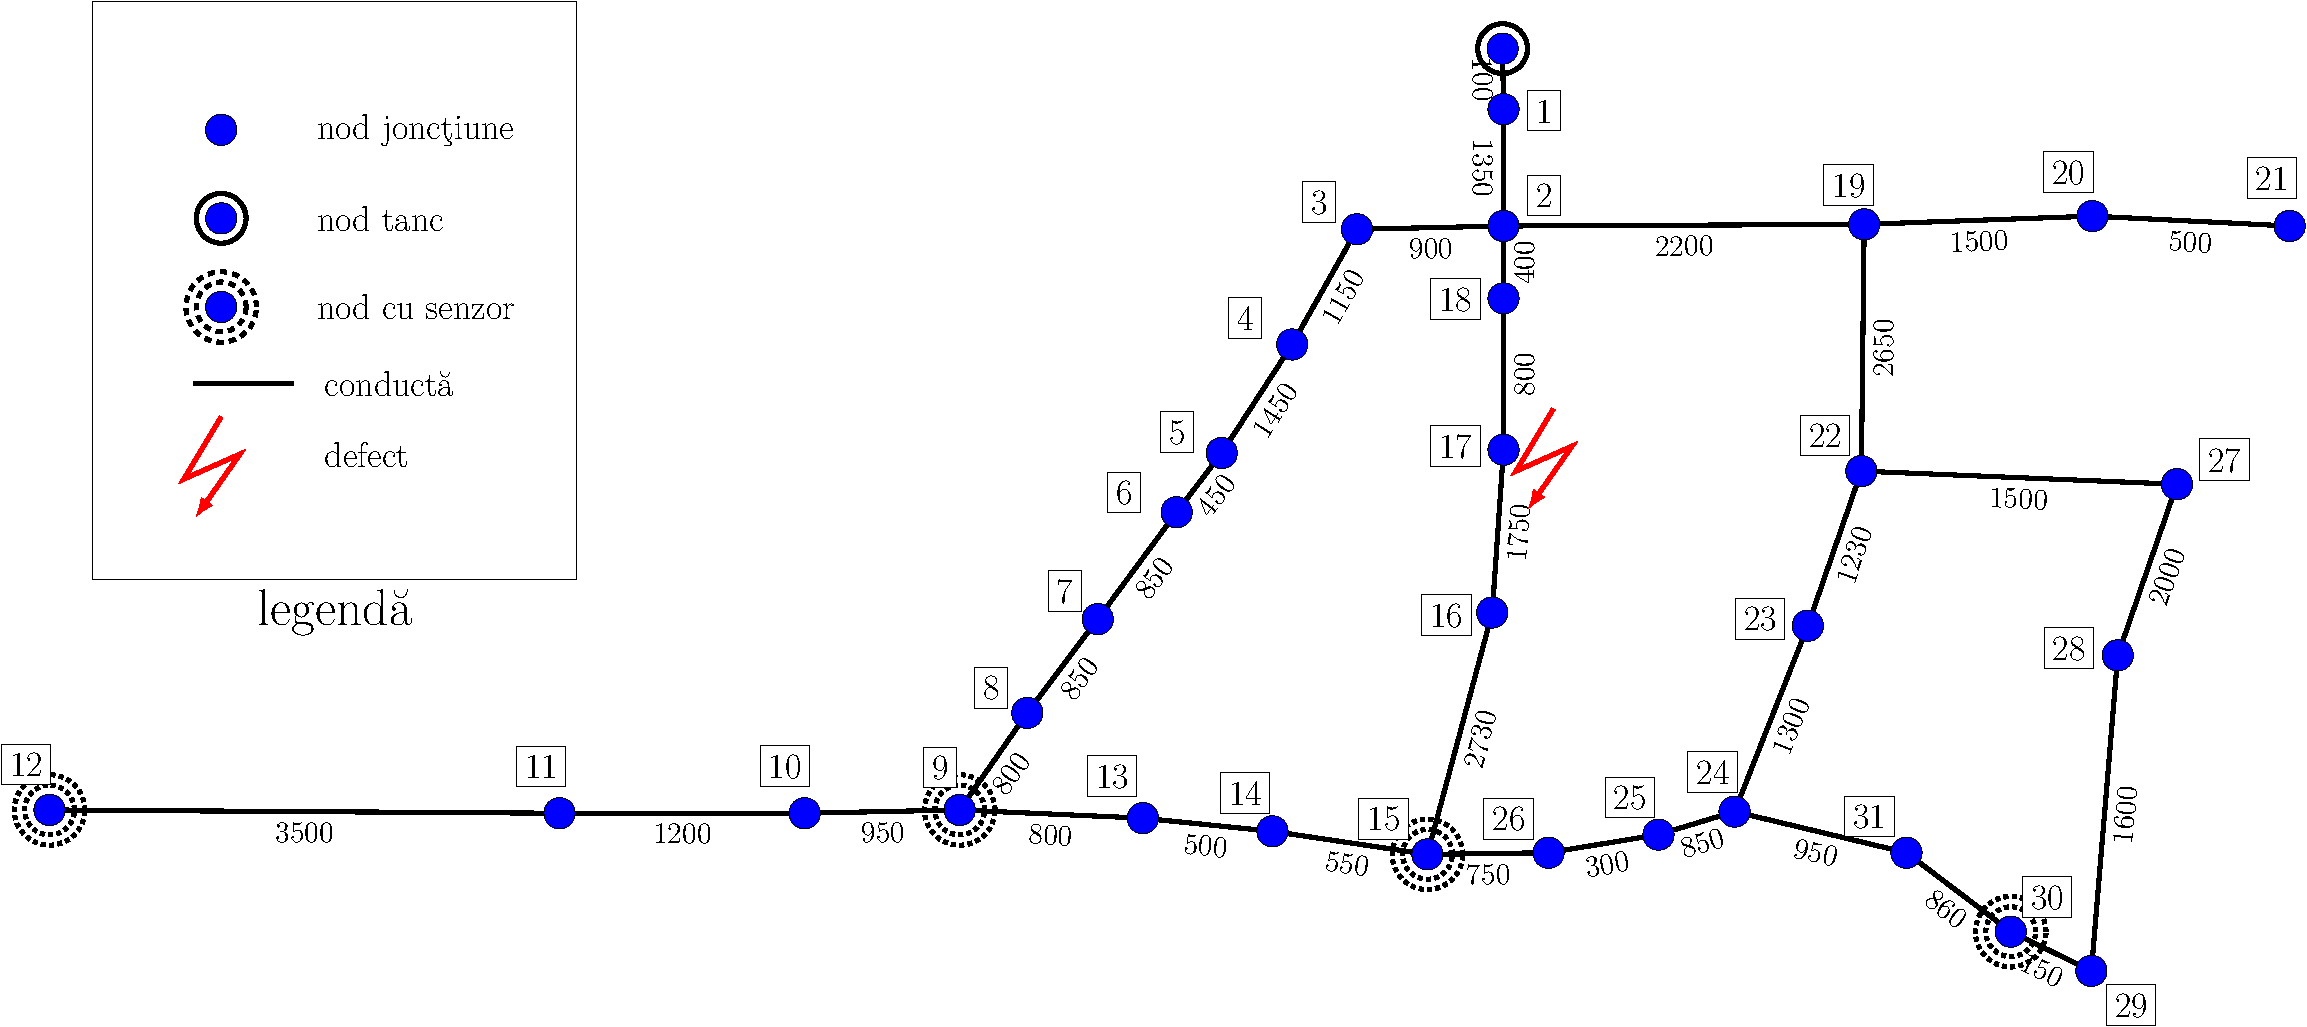
\includegraphics[width=\textwidth]{pics/c1_pics/hanoi_network.pdf}
\caption{Graful rețelei de apă din Hanoi \cite{irofti2017dictionary}}
\label{fig:hanoinetwork}
\end{figure}

După cum se poate observa în figura de mai sus au fost reprezentate două tipuri de node pasive, anume tancurile și joncțiunile. În cazul apariției unui defect în rețea, este important de luat în considerație modalitatea în care acesta va influența valorile apărute în rețea, spre exemplu este de la sine înțeles că dacă se cosideră un defect în nodul cu indicele 17 - i.e. în acest nod au apărut anumite scurgeri care afectează fluxul de apă către consumatori - nodurile în care se va observa o modificare puternică a caracteristicilor (presiune și debit) vor face parte din mulțimea nodurilor adiacente rețelei $S=\{V_{16}, V_{18}\}$, deși pare o concluzie naturală, o modelare matematică riguroasă din care să se tragă această nu este o problemă ușor de rezolvat, anumiți parametrii fiind extrem de greu de estimat chiar și în cazul în care se consideră un regim staționar.

\chapter{Simulări și software folosit}
\label{chap:simulari}

\section{Dificultatea estimărilor parametrilor într-o rețea de apă}

Găsirea unui set de ecuații al cărei soluție să conducă la o estimare îndeajuns de bună pentru control este o condiție sine qua non pentru detecția unui defect și izolarea acestuia în cadrul nodurilor rețelei. Astfel după cum a fost expus în capitolul \ref{chap:intro} ecuațiile care guvernează relațiile intre viteza prin conducte și presiune dintr-un anumit punct sunt particularizări ale ecuațiilor Bernoulli-Euler sau Navier-Stokes. În cadrul unei rețele de apă a unui oraș, complexitatea rezolvării problemei crește semnificativ din varii motive precum:
\begin{itemize}
\item ansamblul de coduncte și noduri interconectate dă naștere unui sistem fizic greu de modelat matematic
\item parametrii care pot influența calitatea soluțiilor precum: tipul materialului conductei și al nodului, elevația fiecărui nod, rugozitatea fiecărei conducte și depunerile de pe aceasta
\item apariția unor factori exogeni care pot fi uneori greu de estimat - tiparul de utilizare al rețelei de către consumatori poate varia puternic
\item apariția defectelor precum scurgerile în proximitatea unui nod
\end{itemize}

Ținând cont de complexitatea problemei în regim dinamic pentru a putea obține o soluție de regim staționar a rețelei este necesar să ignorăm evenimentele imprevizibile precum apariția unei scurgeri sau variațiile bruște ale consumului.

Ecuațiile de regim staționar includ condiții de conservare fluxului de apă:

\begin{equation}
\label{Ecuația de conservare a rețelei de apă}
\sum\limits_{j=1}^{n} \mathbf B_{ij}\mathbf q_j=\mathbf d_i
\end{equation}

Unde $q_i$ reprezintă debitul prin fiecare conductă iar \textbf{B} reprezintă matricea de adiacență a rețelei la echilibru, definită astfel
\begin{equation}
\textbf{B}_{ij} = 
     \begin{cases}
       1, & \text{conducta j intră în nodul i}\\
       0, & \text{conducta j nu este conectată la nodul i} \\
       -1, & \text{conducta j iese din nodul i}\\ 
     \end{cases}
\end{equation}

Partea de estimare a diferenței de presiuni (în engl. "Head-Flow differential") între două noduri interconectate se face utilizând formula Hazen-Williams \cite{sanz2016demand}:
\begin{equation}
\label{debit_presiune}
\mathbf h_i-\mathbf h_j=\frac{10.67\cdot L_\ell}{C_\ell^{1.852}\cdot D_\ell^{4.87}}\cdot \mathbf q_\ell\cdot |\mathbf q_\ell|^{0.852}
\end{equation}

unde:
\begin{itemize}
\label{Hazen-Williams}
\item $\textbf{h}$ reprezintă presiunea - măsurată de obicei în metru coloană de apă
\item $C_l$  reprezintă coeficientul de rugozitate al conductei
\item $D_l$ reprezintă diametrul conductei
\item $L_l$ reprezintă lungimea conductei
\item $q_l$ reprezintă debitul
\end{itemize}

Din ecuația empirică \eqref{Hazen-Williams} termenul $R_{ij}=\frac{10.67\cdot L_\ell}{C_\ell^{1.852}\cdot D_\ell^{4.87}}$ reprezintă rezistența conductei $ij$ iar dual, putem obține conductivitatea conductei $G_{ij} = \frac{1}{R_{ij}}$

Având la dispoziție \eqref{Hazen-Williams} și \eqref{debit_presiune} putem exprima dependența debit presiune în regim staționar sub o formă matriceală compactă și cu o structură neliniară:

\begin{equation}
\mathbf B\mathbf G\left[\left(-\mathbf B^\top \mathbf h+\mathbf B_f^\top \mathbf h_f\right)\times \left|-\mathbf B^\top \mathbf h+\mathbf B_f^\top \mathbf h_f\right|^{-0.46}\right]=\mathbf d
\end{equation}

unde s-au luat în calcul și nodurile care au variații de presiune foarte mici - spre exemplu nodurile de tip tanc și  nodurile de tip rezervor - termenul $\mathbf B_f^\top \mathbf h_f$ reprezintă contribuția acestor noduri la starea de echilibru a rețelei.

Din cauza dificultății rezolvării unei ecuații matriceale neliniare, software-ul specializat trebuie să folosească diferite metode de optimizare ("Solver") pentru a putea obține o diferență cât mai mică între cazul estimat și rezultatul real al ecuației. Este important de reținut faptul că rezolvarea problemelor de programare neliniară cu constrângeri poate generea de fapt o problemă NP-completă, sau în unele cazuri chiar NP-dură \cite{karp1975computational}.

\section{Simulări folosind biblioteca EPANET}
\chapter{Detecția și izolarea defectelor}
\label{chap:detectie}
\section{Definirea defectelor}
Defectele sunt simulate modificând parametrul $C$ din ecuația emitter-ului \eqref{eq:emitter}. Modalitatea prin care se execută în cod simularea unui defect este prin apelarea metodei:

\lstinputlisting[language=Python, caption={Funcție pentru simularea defectelor},label={lst:set_emitter}, firstline=23,lastline=26]{\code/ENWrapper.py}

parametrii funcției $set\_emitter$ sunt:
\begin{itemize}
\item node\_inde - indexul nodului în care se simulează defectul
\item emitter\_val - magnitudinea defectului
\end{itemize}

Metoda mai întâi vefică dacă nodul cu indexul $node_index$ reprezintă doar o jonncțiune apoi setează magnitudinea defectului în nodul primit cu ajutorul funcției de bibliotecă $\mathbf{ENsetnodevalue}$ 

\section{Simulare dinamică pentru defecte în diferite noduri}

În continuare vom considera un scenariu de defect pentru rețea care constă în modificarea succesivă a parametrului de proporționalitate din relația de calcul a debitului de emitter \eqref{eq:emitter}. În imaginile următoare voi considera mai multe magnitudini de defect într-un anumit nod și voi reprezenta grafic răspunsul în timp al rețelei în același nod.

\begin{figure}[H]

\subfloat[Profile cu defect în nodul 14]{%
  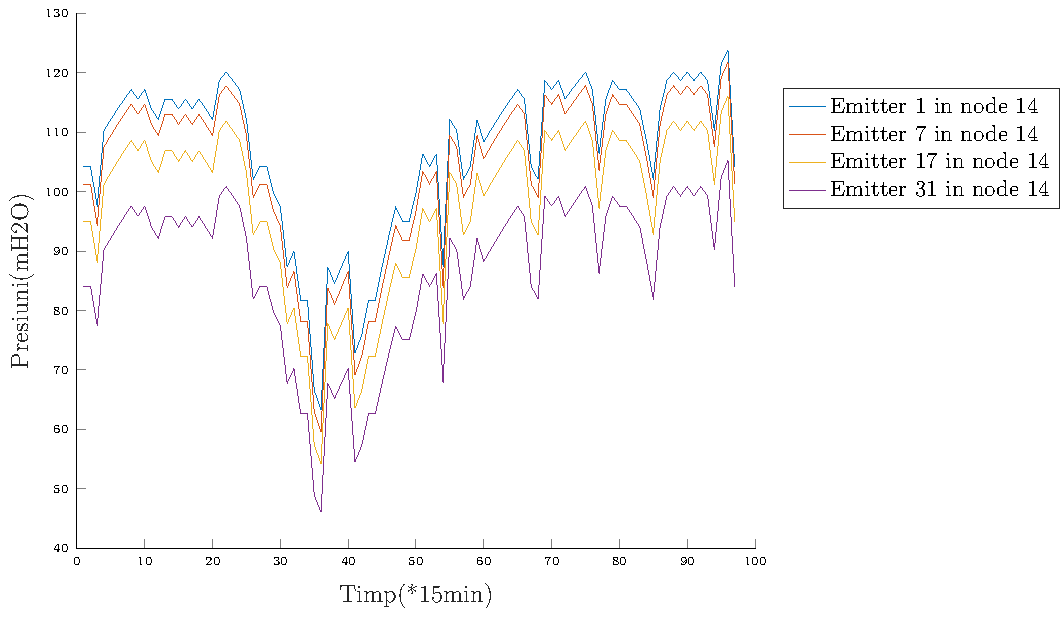
\includegraphics[width=0.5\textwidth]{\pics/c3_pics/emitter_node_same/emitter_node14}%
  \label{fig:emitter_node_same14}%
}\qquad
\subfloat[Profil cu defect în nodul 25]{%
  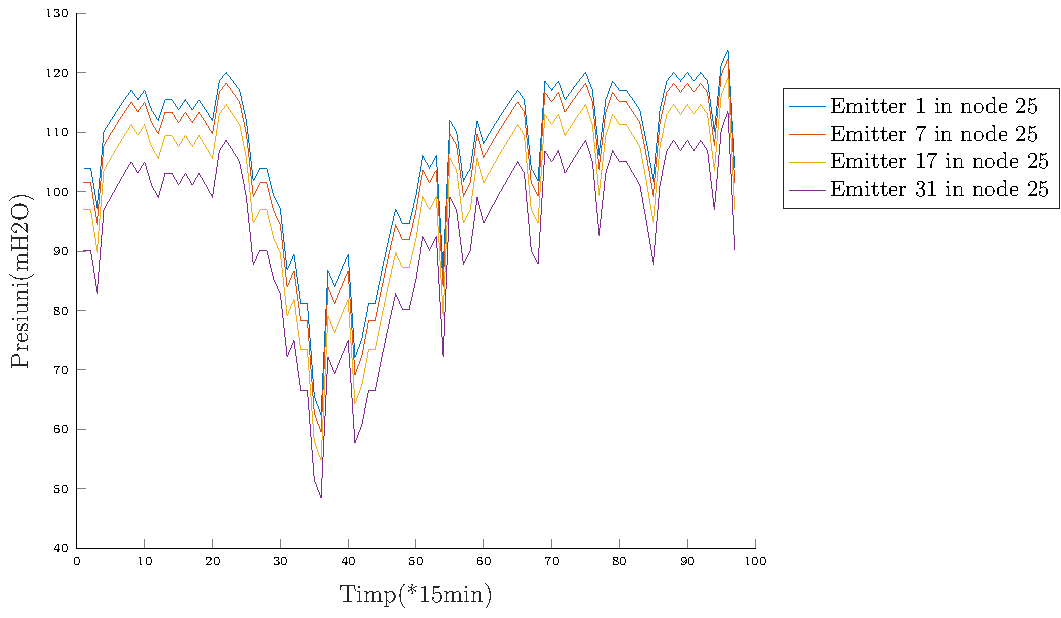
\includegraphics[width=0.5\textwidth]{\pics/c3_pics/emitter_node_same/emitter_node25}%
  \label{fig:emitter_node_same25}\qquad
}

\caption{Rezultate simulări defecte ușoare}
\label{fig:ref_emitter_soft}
\end{figure}

După cum se poate observa în imaginile \ref{fig:ref_emitter_soft} variația emitter-ului într-un nod produce în mod evident o modificarea a modului comun al caracteristicii $timp-presiune$. Din punctul de vedere al magnitudinolor de simulare pentru defecte, am considerat 2 clase de defecte, anume:
\begin{itemize}
\item defecte ușoare (soft faults) - cu valorile coeficientului de emitter mai mici de 35
\item defecte puternice (hard faults) - cu valorile emitter mai mari de 35 
\end{itemize}

Cele din urmă produc și modificări ale caracteristicii dinamice, introducând distorsiuni sau aplatizări ale mărimilor măsurate. Reprezentarea defectelor hard este reprezentată în figurile de mai jos:

\begin{figure}[H]

\subfloat[Profile cu defect puternic în nodul 14]{%
  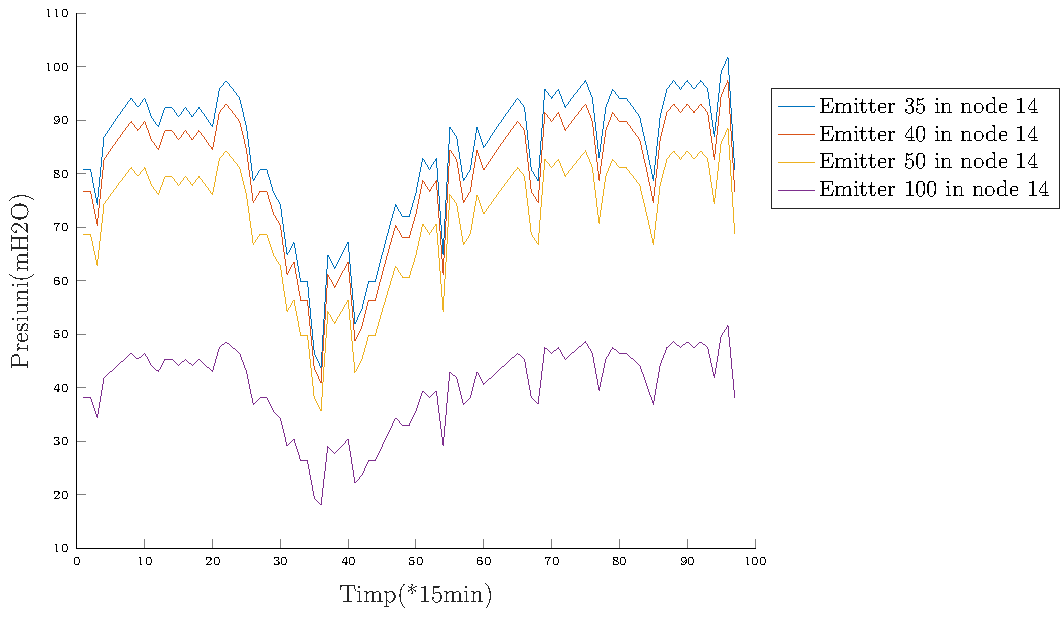
\includegraphics[width=0.5\textwidth]{\pics/c3_pics/emitter_node_same/emitter_hard_node14}%
  \label{fig:emitter_hard_node_same14}%
}\qquad
\subfloat[Profil cu defect puternic în nodul 25]{%
  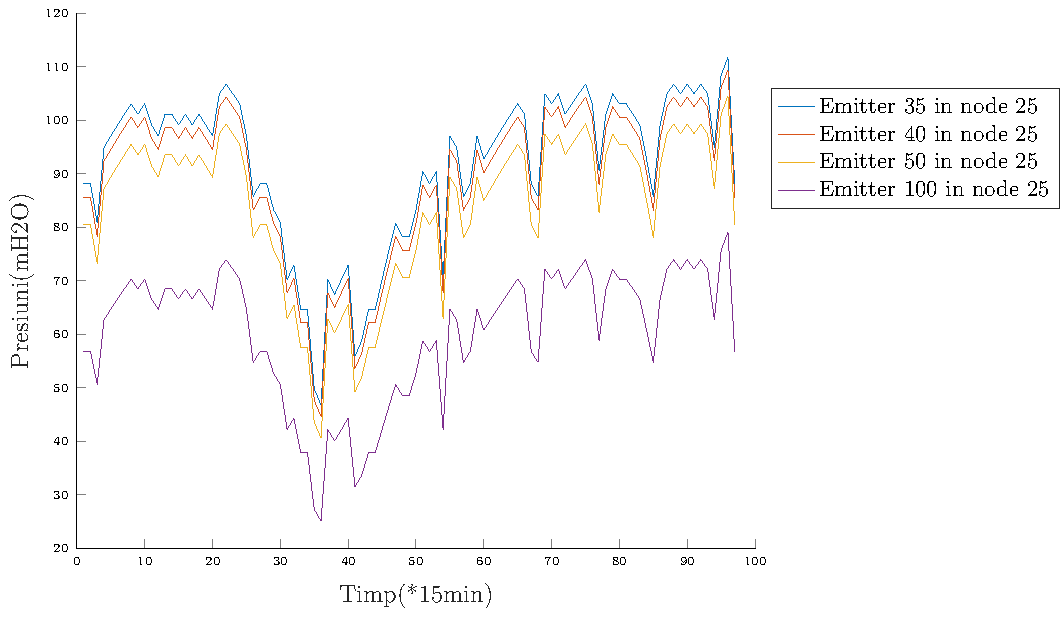
\includegraphics[width=0.5\textwidth]{\pics/c3_pics/emitter_node_same/emitter_hard_node25}%
  \label{fig:emitter_hard_node_same25}\qquad
}
\caption{Rezultate simulări defecte puternice}
\label{fig:ref_emitter_hard}
\end{figure}

Se observă de exemplu că pentru o valoare a emitter-ului de 100 caracteristica dinamică este deja modificată din cauza scurgerilor puternice din nod. 

Este relevantă împărțirea defectelor în mai multe clase de magnitudini pentru a putea valida un model de clasificare. Spre exemplu este normal să se întrebe dacă un model antrenat pe baza unui set date corespunzător unor magnitudini normale $C \in (0, 35)$ poate da rezultate semnificative pentru un set de date cu magnitudini ale emitter-ului puternice $C \geqslant 35$. 

\section{Preprocesarea datelor}
\label{sec:preproc}
În urma extragerii datelor din rețea este extrem de importantă etapa de prelucrare și preprocesare a datelor. Domeniul de preprocesare a datelor este unul extrem de vast și important în domeniul de învățare automată (engl. Machine Learning) și procesare de semnal. Preprocesarea datelor este etapa în care datele de intrare pentru un algoritm sunt aduse la o formă optimă pentru desfășurarea procesului impus, de exemplu în domeniul clasificării este important ca algoritmii să primească date care să fie scalate într-un anumit domeniu, pentru a asigura convergența\cite{dataPreprocessing}, \cite{GIGO}. Alegerea metodei de preprocesare este strâns legată de tipul de date disponibile și de starea acestora. În cazul rețelelor de apă, unde am ales caracteristica presiunii ca mărime de intrare pentru algoritm și ținând cont de răspunsul în timp al rețelei am considerat ca fiind necesare următoarele operații:

\begin{itemize}
\item eliminarea frontului comun și extragerea diferenței dintre semnalul nominal și cel măsurat în rețea
\item filtrarea semnalului obținut anterior
\end{itemize}

\section{Nomenclatura mărimilor alese}
\label{sec:nomenclatura}
Pentru a menține rigurozitatea și eleganța metodelor folosite este nevoie de o definire matematică pentru toate mărimile și metodele de filtrare folosite.

\subsection{Presiunea în regim dinamic}
Reprezintă o funcție de timp:
\begin{equation}
p_i : \mathbb{R} \longrightarrow \mathbb{R}^n, i \in V
\label{eq:press:func}
\end{equation}

unde $n$ reprezintă numărul de noduri al rețelei, iar $i$ reprezintă indexul nodului. 
Deoarece cazurile tratate în această lucrare reprezintă momente discrete de timp este important să definim presiunea măsurată în intervalele discrete în care este simulat procesul:
\begin{equation}
\mathbf{p}_i \in \mathbb{R}^{n \times p_{sim}}
\end{equation}

unde $p_{sim}$ reprezintă numărul de eșantioane pentru fiecare măsurătoare. Mergând mai departe în analiza simulării este de asemenea important să definim mărimea afectată de un defect în nodul $j$, de magnitudine $m$ și măsurată în nodul $i$:
\begin{equation}
\mathbf{p}^{j,m}_i \in \mathbb{R}^{n \times p_{sim}}
\end{equation}

Pentru cazul în care magnitudinea $m$ ia valori nule, atunci vom considera notația mărimii nominale:
\begin{equation}
\mathbf{p}^{j,0}_i = \mathbf{p}^{nom}_i, \forall j \in V
\end{equation}

Pentru valorile presiunii recoltate din rețea în nodul $i$ despre care nu se cunoaște nici o informație, vom considera notația
\begin{equation}
\widehat{\mathbf{p}}_i
\end{equation}

\subsection{Presiunea în regim static}
Considerând o plajă de momente de timp situate între indicii $rs_1 : rs_2$ unde se afla valorile de regim staționar ale procesului, putem defini o medie a regimului static în felul următor:
\begin{equation}
\overline{\mathbf{p}}_i^{j,m} = \frac{1}{rs_1 - rs_2 + 1} \sum_{k=rs_1}^{rs_2} \mathbf{p}_i^{j,m}[k] 
\label{eq:pmean}
\end{equation}

În aceeași manieră definim și media presiunii nominale în regim static:
\begin{equation}
\overline{\mathbf{p}}_i^{j,0} = \overline{\mathbf{p}_i}^{nom}, \forall j \in V
\label{eq:pmean_nom}
\end{equation}

Media presiunii măsurată în nodul $i$ și despre care nu se cunosc informații în legătură cu valoarea și poziția defectului:
\begin{equation}
\overline{\widehat{\mathbf{p}}}_i = \frac{1}{rs_1 - rs_2 + 1} \sum_{k=rs_1}^{rs_2} \widehat{\mathbf{p}}_i^[k] 
\label{eq:pmean_measured}
\end{equation}

\subsection{Reziduuri}
Așa cum a fost discutat în secțiunea \ref{sec:preproc}, preprocesarea datelor are un rol important iar în cazul analizei și clasificării defectelor în rețelele cu apă, este nevoie să definim caracteristica prelucrată care va fi folosită mai apoi în procesul de izolare a defectelor. Reziduul absolut reprezintă diferența dintre valoarea măsurată în rețea și valoarea nominală, aici putem discerne două cazuri:
Reziduu temporal:
\begin{equation}
\mathbf{r}_i^{j,m} = \mathbf{p}_i^{j,m} - \mathbf{p}_i^{nom}
\label{eq:temp_residual}
\end{equation}
Reziduu atemporal, calculat ca diferența dintre cele două valori mediate pe intervalul staționar al caracteristicii:
\begin{equation}
r_i^{j,m} = \overline{\mathbf{p}}_i^{j,m} - \overline{\mathbf{p}}_i^{nom}
\label{eq:absolute_residual}
\end{equation}

iar pentru valorile reziduului despre care nu se cunosc încă lucruri folosim notația din stilul anterior:
\begin{equation}
\widehat{r}_i = \overline{\widehat{\mathbf{p}}}_i - \overline{\mathbf{p}}_i^{nom}
\label{eq:measured_residual}
\end{equation}

Alte tipuri de reziduuri preprocesate sunt relative:
\begin{equation}
rrelativ_i^{j,m} = \frac{r_i^{j,m}}{\overline{\mathbf{p}}_i^{nom}} 
\label{eq:relative_residual}
\end{equation}

Reziduurile normate:
\begin{equation}
rnorm_{i}^{j,m} =  \frac{r_i^{j,m}}{ \norm{r_{1:n}^{j,m}}} 
\label{eq:norm_residual}
\end{equation}

Reziduurile scalate:
\begin{equation}
rscal_{i}^{j,m} = \frac{r_i^{j,m} - \min r_{1:n}^{j,m}}{ \max r_{1:n}^{j,m} -  \min r_{1:n}^{j,m}}
\label{eq:scaled_residual}
\end{equation}


Ca semnificație notațiile prezentate în \ref{sec:nomenclatura} care conțin simbolul~ $\widehat{}$~ fac referire la datele folosite pentru validarea modelului iar valorile unde se specifică nodul defectului și magnitudinea acestuia sunt considerate ca fiind date de antrenare și testare. Astfel în contextul definirii setului de dat pe care vom aplica algoritmii de calsificare va trebui să definim matricea:
\begin{equation}
\mathbf{R}<tip>^{j, m} \in \mathbb{R}^{n_{d} \times n}
\label{eq:residual_mat}
\end{equation}

Unde croșetele din formulă reprezintă un înlocuitor pentru metoda de reziduu folosită iar $n_{d}$ reprezintă numărul de defecte tratate în setul de date. De asemenea pentru fiecare linie a matricei \eqref{eq:residual_mat} putem defini perechea
\begin{equation}
\left( \mathbf{R}<tip>(d,:), y_{d} \right)
\label{eq:residual_mat_label}
\end{equation} 
Unde $ \mathbf{R}<tip>(d,:)$ reprezintă răspunsul rețelei prin reziduuri la defectul $d$. Iar $y_{d}$ reprezintă eticheta pentru acest set de date, anume, nodul în care a avut loc defectul.

\section{Calcul și prezentare reziduuri}
În continuare vom prezenta grafic reziduurile temporale normalizate care apar în rețea pentru diferite scenarii ale defectelor definite anterior.
Astfel vom considera nodurile de măsurătoare ca o submulțime  a lui $V' \subset V$ și $ V = \{5, 11, 15, 17, 21, 27\}$, nodurile în care s-au simulat defecte sunt $V_{d} = \{11, 17, 27,29\}$.

 
\begin{figure}[H]
\begin{tabular}{cc}
\subfloat[Reziduuri pentru defect în nodul 11, magnitudine 29]{%
  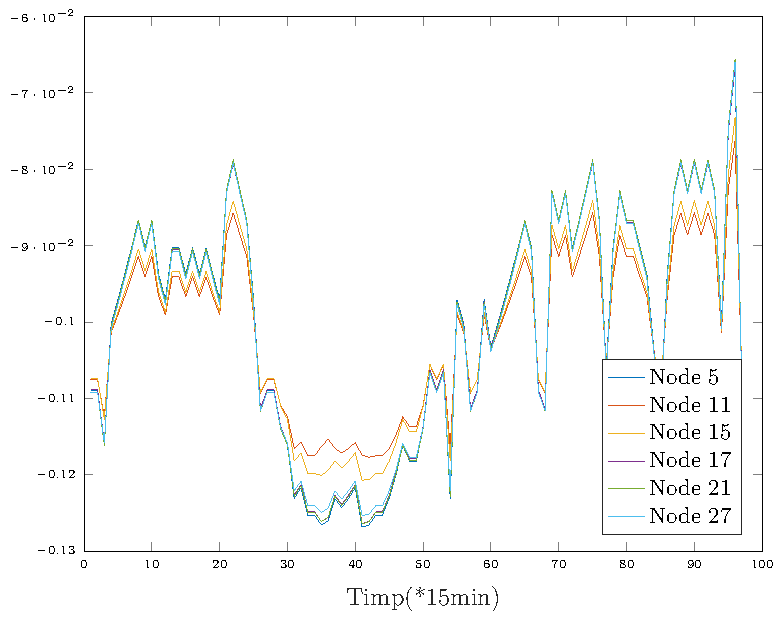
\includegraphics[width=0.5\textwidth]{\pics/c3_pics/residuals/time_res_emitter11_mag29}%
  \label{fig:residual_time_11}%
} &
\subfloat[Reziduuri pentru defect în nodul 17, magnitudine 29]{%
  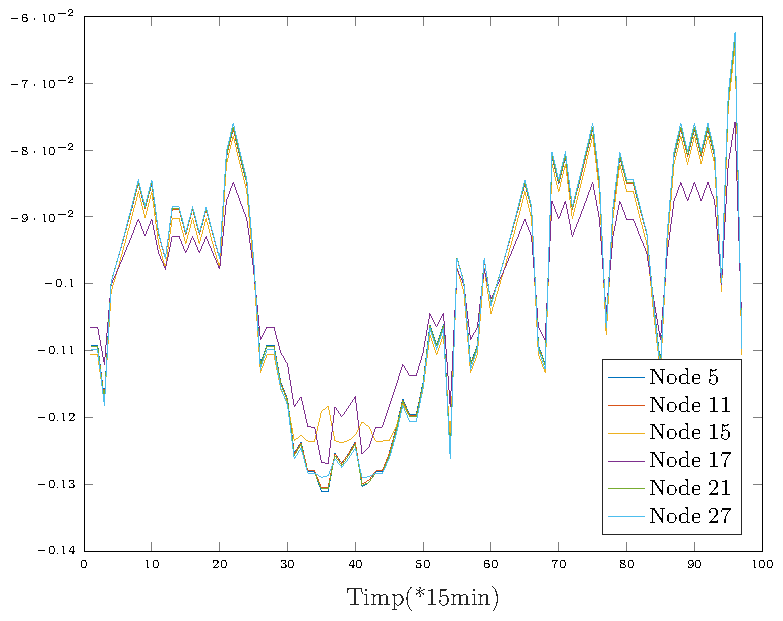
\includegraphics[width=0.5\textwidth]{\pics/c3_pics/residuals/time_res_emitter17_mag29}%
  \label{fig:residual_time_17}%
} \\

\subfloat[Reziduuri pentru defect în nodul 21, magnitudine 29]{%
  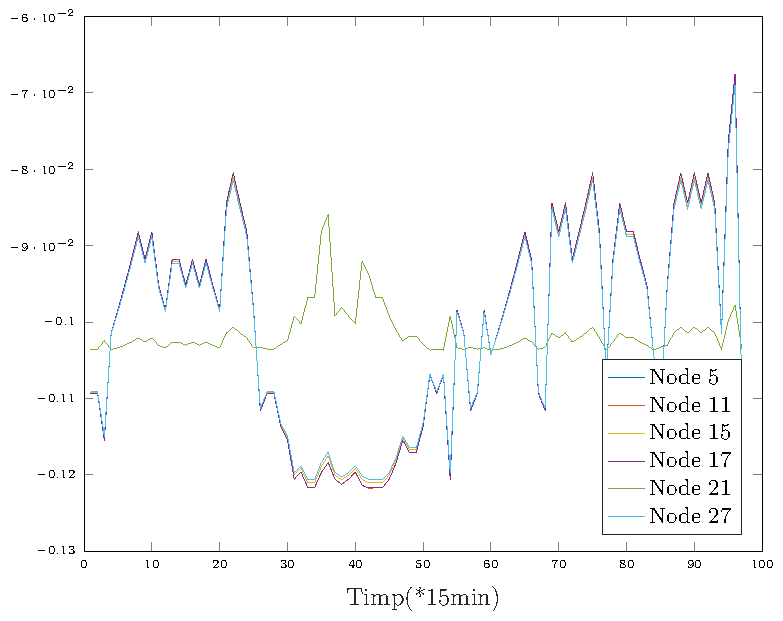
\includegraphics[width=0.5\textwidth]{\pics/c3_pics/residuals/time_res_emitter21_mag29}%
  \label{fig:residual_time_21}%
}&

\subfloat[Reziduuri pentru defect în nodul 27, magnitudine 29]{%
  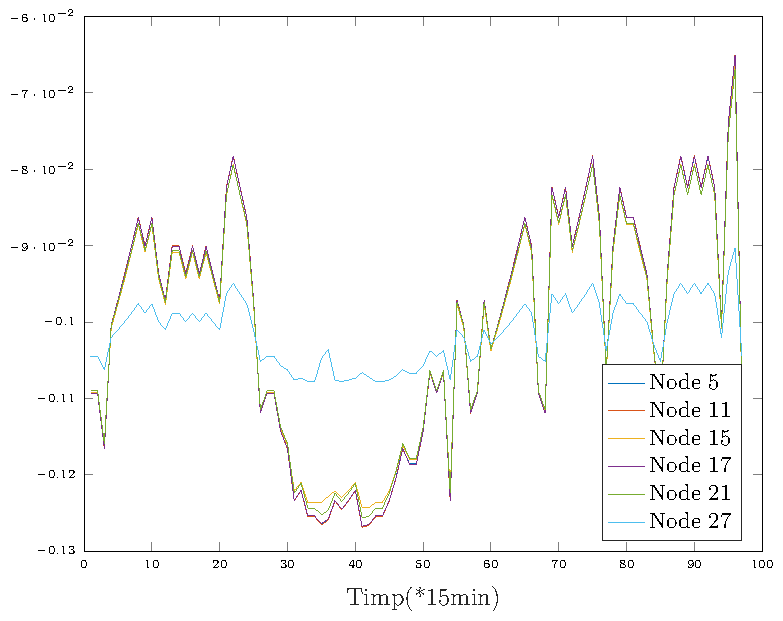
\includegraphics[width=0.5\textwidth]{\pics/c3_pics/residuals/time_res_emitter27_mag29}%
  \label{fig:residual_time_27}%
} 
\end{tabular}
\caption{Reziduuri rețea}
\label{fig:rez_time}
\end{figure}


Se poate observa că în figurile \ref{fig:rez_time} reziduul cel mai pronunțat ca funcție de timp se găsește în nodul în care se simulează și defectul - lucru natural și de așteptat. O caracteristică importantă a acestei rețele de apă este faptul că există o dependență între diferitele răspunsuri în timp ale caracteristicii de presiune, fapt care ne permite să exploatăm redundanțele din rețea și să prezicem cu o acuratețe relativ ridicată defectele.

Este necesar acum să prezentăm profilurile reziduurilor atemporale, care în final vor reprezenta caracteristicile de intrare pentru algoritmul de clasificare și selecție de senzori.

\begin{figure}[H]
\begin{tabular}{cc}
\subfloat[Reziduuri pentru defect în nodul 11, magnitudine 25]{%
  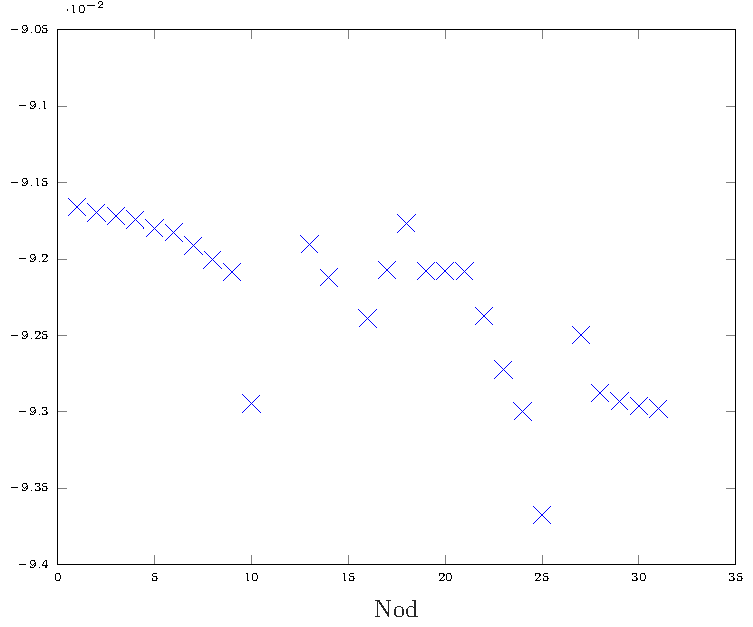
\includegraphics[width=0.5\textwidth]{\pics/c3_pics/residuals/atem_res_emitter11_mag25}%
  \label{fig:residual_atemp_11}%
} &
\subfloat[Reziduuri pentru defect în nodul 17, magnitudine 25]{%
  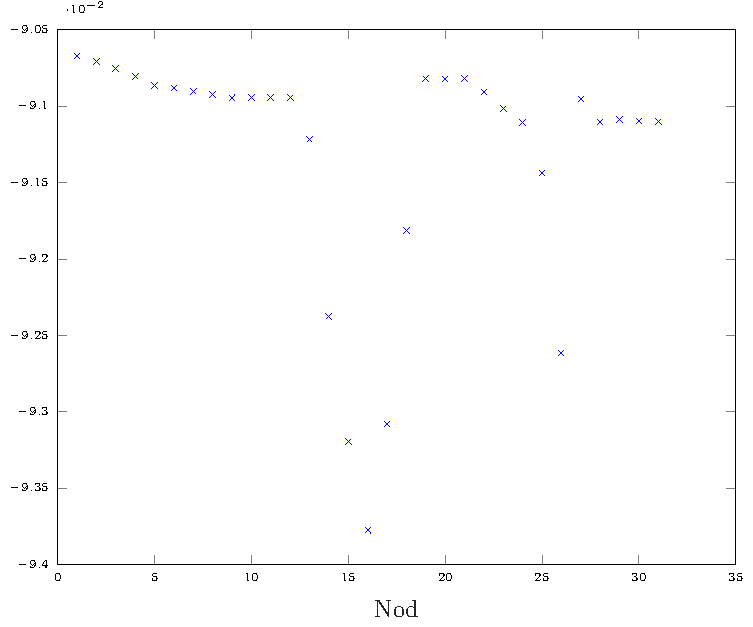
\includegraphics[width=0.5\textwidth]{\pics/c3_pics/residuals/atem_res_emitter17_mag25}%
  \label{fig:residual_atemp_17}%
} \\

\subfloat[Reziduuri pentru defect în nodul 21, magnitudine 25]{%
  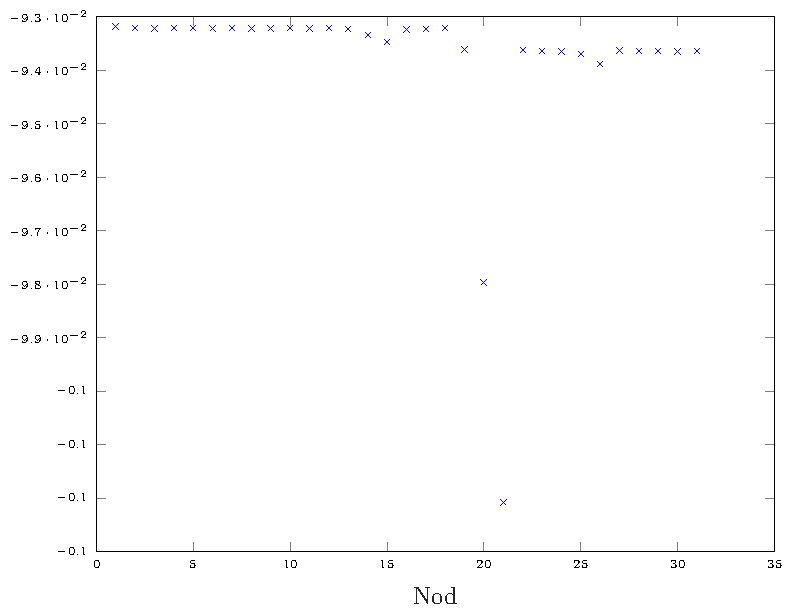
\includegraphics[width=0.5\textwidth]{\pics/c3_pics/residuals/atem_res_emitter21_mag25}%
  \label{fig:residual_atemp_21}%
}&

\subfloat[Reziduuri pentru defect în nodul 27, magnitudine 25]{%
  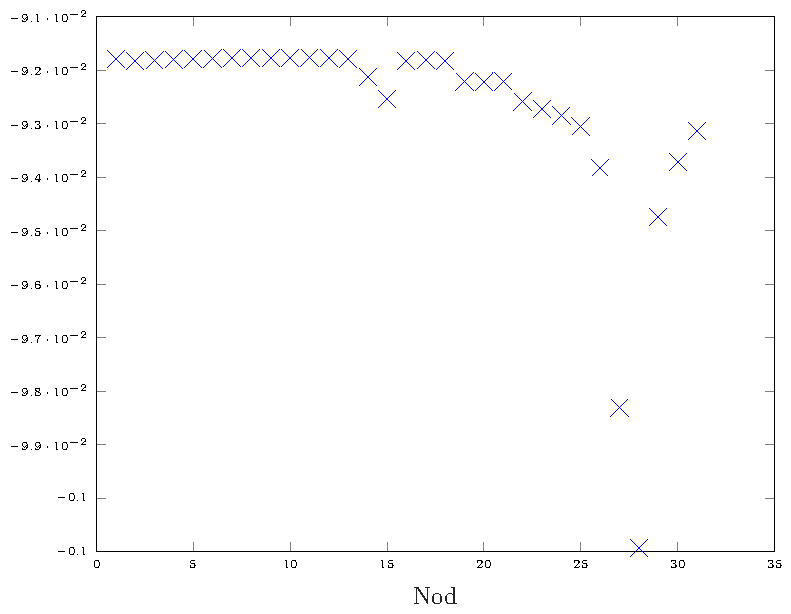
\includegraphics[width=0.5\textwidth]{\pics/c3_pics/residuals/atem_res_emitter27_mag25}%
  \label{fig:residual_atemp_27}%
} 
\end{tabular}
\caption{Reziduuri atemporale rețea}
\label{fig:rez_atemp}
\end{figure}

Asemenea reziduurilor de la \ref{fig:rez_time} se poate observa că simularea unui emitter într-un nod va determina un răspuns puternic în nodul respectiv și în vecinătatea nodului afectat

\section{Metodă preliminară de selecție a senzorilor}
O metodă prin care se poate decide și evalua importanța senzorilor într-o rețea este prin construirea matricei de reziduuri \eqref{eq:residual_mat}, asupra căreia aplicăm o operație de scalare pe coloane, pentru a aduce valorile acesteia în intervalul $[0,1]$. Pentru experimentul în care simulăm în fiecare nod un emitter de 25 obținem grafic o matrice $\mathbf{R}scaled \in \mathbb{R}^{31 \times 31}$:

\begin{figure}[H]
\centering

\includegraphics[width=0.5\textwidth]{\pics/c3_pics/residuals/residual_scaled_matrix}
\caption{Matricea de reziduuri scalate}
\label{fig:rez_scaled_matrix_img}
\end{figure} 

După cum se observă în \ref{fig:rez_scaled_matrix_img} fiecare coloană a matricei $\mathbf{R}scaled$ reprezintă răspunsul prelucrat - scalat în intervalul $[0,1]$ - al unui defect, valorile care tind spre o culoare mai închisă de negru sunt răspunsuri mai pronuțate iar valorile care se apropie de alb reprezintă valori mai puțin evidențiate ale reziduului în nod. Analizând matricea se poate observa care noduri răspund mai bine la anumite răspunsuri, o caracteristică importantă a acestei matrice este că, o alură diagonală - semnificația elementelor diagonale fiind răspunsul nodurilor afectate de defecte aplicate în ele însuși. Dacă matricea de reziduuri ar fi avut o caracteristică diagonală perfectă - elementele nenule s-ar fi regăsit doar pe aceasta - problema de clasificare ar fi fost una simplă și ar fi implicat amplasarea unui senzor în fiecare nod. Cazul real impune dependențe între presiunile, debitele din fiecare nod, dar și vitezele din fiecare conductă, astfel, fiecare defect separat va avea o "amprentă" unică - prin care se diferențiază de celelalte și una comună. Scopul este găsirea unui subset al mulțimii de noduri care să poată identifica defectele cu pierderi minime de performanțe.


\subsection{Binarizarea matricei de reziduuri}

bla bla


%%%%%%%%%%%%%%%%%%%%%% back matter %%%%%%%%%%%%%%%%%%%%%%%%%%%%%%%%%%%%%%
\appendix
\appendixpage
%\addappheadtotoc
\begin{appendices}																				  % from here onwards are the appendices
%\chapter{Notaţii matematice consacrate}
\label{chap:not}

\begin{description}[style=nextline]
\item[Constante scalare] $\mathrm{a}$, $\mathrm{A}$, $\mathrm{b}$, $\mathrm{B}$, $\mathrm{c}$, $\mathrm{C}$ etc. (litere normale, cu precădere din prima parte a alfabetului);
\item[Constante vectoriale] $\mathbf{a}$, $\mathbf{b}$, $\mathbf{c}$ etc. (litere minuscule, aldine (\textbf{bold}), cu precădere din prima parte a alfabetului);
\item[Constante matriciale] $\mathbf{A}$, $\mathbf{B}$, $\mathbf{C}$, $\mathbf{P}$, $\mathbf{Q}$, $\mathbf{R}$ etc. (litere majuscule, aldine (\textbf{bold}), cu precădere din zona alfabetului unde nu se afl\u a litere alocate în mod tradi\c tional indicilor);
\item[Variabile scalare] $x$, $y$, $z$  etc. (aplecate (\emph{italic}), ne-aldine, cu prec\u adere din ultima parte a alfabetului);
\item[Variabile vectoriale] $\mathbf{x}$, $\mathbf{y}$, $\mathbf{z}$ etc (litere minuscule, aldine (\textbf{bold}), cu precădere din ultima parte a alfabetului);
\item[Variabile  matriciale]  $\mathbf H(q^{-1})$, $\mathbf H(s)$, $\mathbf H(z)$, $\mathbf H(t)$, $\mathbf H[k]$ etc. (litere  majuscule,  aldine (\textbf{bold}), cu unul sau mai multe argumente scalare sau vectoriale);
\item[Operatori]  $\min$ (minim), $\max$ (maxim), opt (optim), $\arg$ opt (argument de optimizare sau punct de optimizare), $q^{-1}$  (întârziere), $Tr$ (urmă (\emph{trace})), $Tz$ (Toeplitz), $Pr$ (proiec\c tie) etc, (litere normale, urmate obligatoriu de explica\c tia privind nota\c tia, la prima utilizare);
\item[Timp continuu] $t\in \mathbb R$;
\item[Timp discret] $n\in \mathbb Z$ sau $k\in \mathbb Z$;
\item[Argument de timp continuu] $(t)$ (între parenteze rotunde);
\item[Argument de timp discret] $[n]$ (între paranteze drepte);
\item[Număr de itera\c tie sau indici] $i$, $j$, $k$, $l$, $m$, $n$  etc. (aplecate, cu precădere din partea de mijloc a alfabetului); exemplu de nota\c tie complex\u a": $x_i^k[n]$ -- componenta $i$ a vectorului $\mathbf x$, la momentul discret $n$, pentru iteratia $k$;
\item[Caractere greceşti frecvent utilizate (în ordinea firească a alfabetului grecesc)]~
\begin{itemize}
\item $\alpha$ (/alfa/, \verb+\alpha+)
\item $\beta$ (/beta/, \verb+\beta+)
\item $\gamma$, $\Gamma$ (/gama/, \verb+\gamma, \Gamma+)
\item $\delta$, $\Delta$ (/delta/, \verb+\delta, \Delta+)
\item $\epsilon$ (/epsilon/, \verb+\epsilon+)
\item $\zeta$ (/\c teta/, \verb+\zeta+)
\item $\eta$ (/ita/, \verb+\eta+)
\item $\theta$, $\Theta$ (/teta/, \verb+\theta, \Theta+)
\item $\kappa$ (/kapa/, \verb+\kappa+)
\item $\lambda$, $\Lambda$ (/lambda/, \verb+\lambda, \Lambda+) a nu se pronun\c ta /lamda/
\item $\mu$ (/miu/, \verb+\mu+)
\item $\nu$ (/niu/, \verb+\nu+)
\item $\xi$ (/xi/, \verb+\xi+)
\item $\pi$, $\Pi$ (/pi/, \verb+\pi, \Pi+)
\item $\rho$ (/ro/, \verb+\rho+)
\item $\sigma$, $\Sigma$ (/sigma/, \verb+\sigma, \Sigma+)
\item $\tau$ (/tau/, \verb+\tau+)
\item $\phi$, $\varphi$, $\Phi$ (/fi/, \verb+\phi, \varphi, \Phi+)
\item $\chi$ (/hi/, \verb+\chi+)
\item $\psi$, $\Psi$ (/psi/, \verb+\psi, \Psi+)
\item $\omega$, $\Omega$ (/omega/, \verb+\omega, \Omega+)
\end{itemize}
Şi  în  cazul  lor,  se  vor  respecta  regulile  de  nota\c tie  pentru  scalari/vectori. % Totuşi,  în  cazul scalarilor, se recomandă ca literele să nu fie scrise aplecat. De exemplu, se va prefera  $\mathrm \alpha$ şi nu $\alpha$.
\item[Alte nota\c tii unificate în Automatică]~
\begin{description}[before={\renewcommand\makelabel[1]{##1 =}},leftmargin=!,labelwidth=\widthof{\bfseries blaaaaaaaa}]
\item[$J$, $\mathbf J$] criteriu (de optimizare), func\c tie-criteriu, (func\c tie) cost, func\c tie economică, func\c tie obiectiv
\item[$u$, $\mathbf u$] intrarea/comanda (scalară sau vectorială a) unui sistem dinamic
\item[$x$, $\mathbf x$] starea (scalară sau vectorială a) unui sistem dinamic
\item[$y$, $\mathbf y$] ieşirea (scalară sau vectorială a) unui sistem dinamic
\item[$v$, $\mathbf v$] perturba\c tia exogenă (scalară sau vectorială) a unui sistem dinamic (asociată cu ieşirile)
\item[$w$, $\mathbf w$] perturba\c tia endogenă (scalară sau vectorială) a unui sistem dinamic (asociată cu stările)
\item[$e$, $\mathbf e$] zgomotul alb (scalar sau vectorial)
\item[$\mathrm{e}$] numărul lui Nepper, baza logaritmului natural (se scrie drept şi nu aplecat)
\item[$s$] variabila (complexă) Laplace
\item[$z$] variabila complexă circulară (specifică Transformatei Z)
\item[$f$, $\mathbf f$] func\c tie neliniară (scalară sau vectorială) asociată în special ecua\c tiei de stare
\item[$g$, $\mathbf g$] func\c tie neliniară (scalară sau vectorială) asociată în special ecua\c tiei de ieşire
\item[$\nabla$, $\nabla_x$] operatorul  de  gradient/Jacobian  (se  pronun\c tă  /nabla/;  \verb+\nabla+);  acest operator se poate nota şi prin $\mathbf J_x$
\item[$\Diamond$, $\Diamond_x$] operatorul  Hessian (se  pronun\c tă  /romb/;  \verb+\Diamond+);  acest operator se poate nota şi prin $\mathbf J_{xx}$
\item[$\mathbf A^T$] transpusa matricii $\mathbf A$
\item[$\bar{\mathbf A}$] conjugata complex\u a a matricii $\mathbf A$
\item[$\bar{\mathbf A}^T$, $A^*$] transpusa  şi  conjugata  complexă  a  matricii $\mathbf A$   (\emph{hermitica}  acesteia);  a  doua nota\c tie poate fi folosită şi pentru a indica doar conjugarea complexă, cu condi\c tia să se men\c tioneze clar de la început semnifica\c tia acesteia
\item[$\mathbf v^R$]  versiunea răsturnată a vectorului  $\mathbf v$  (adică rearanjată prin citirea de jos în sus)
\end{description}
\end{description}
% fisiere sursa

\chapter{Fișiere sursă}
\label{chap:sources}

\lstinputlisting[caption={Cod Matlab -- fișier complet},label={lst:s1}]{\code/s1.m}
\lstinputlisting[caption={Cod Matlab -- fragment de fișier},label={lst:s2},firstline=5,lastline=15]{\code/s2.m}
\end{appendices}

\cleardoublepage

\printbibliography[heading=bibintoc]
\end{document}